\begin{solution}{normal}
First, let us figure out how to calculate the energy cost. It is given in the problem that the electrical energy cost is $c = 0.1\;\mathrm{EUR/kWh}$ so if we find the amount of energy dissipated, we can then convert this to monetary value with using the electricity cost constant via dimensional analysis.
\vspace{3mm}

\noindent Let us make use of idea 4 in Kalda’s handout. If a system is described by a parameter $x$ (which can be time, coordinate, velocity, etc.) and a quantity $A$ can be expressed as $A = \sum_i F_i \Delta x$, where $\Delta x$ is a small interval of the parameter $x$, the sum is taken over all the small intervals, and $F_i$ is a function of $x$. In this case, our parameter is temperature. We divide the graph into small chunks where the temperature at each endpoint of a singular chunk is $T_i$ where $i \in \mathbb{Z}^{+}$. For the cooling period, during the number of days $\Delta N_i$ for which the temperature stayed in the (small) range between $T_i$ and $T_i + \Delta T_i$, the heat loss is $Q_c = (T_i - T_0)C\Delta N_i\cdot 3600\;\mathrm{s/h}$. Note that $(T_i-T_0)\Delta N_i$ is a horizontal narrow rectangular region between the graph and the vertical line $T = T_0$. Therefore, the net energy can be represented as
\[Q_{\text{tot}} = Q_A + Q_B = C\left(\sum_{T_i < T_0} (T_0-T_i) \Delta N_i + \sum_{T_i > T_0} (T_i-T_0) \Delta N_i\right) = C(A_A + A_B)\]where $A_A$ and $A_B$ are the respective areas shown in the graph below. Next, we need to make use of the efficiencies as the total power is not just all we need. Note that when the device is used as an air conditioner (i.e $T_i < T_0$) we use the COP $\eta_c$ and when the device is used to heat the room (i.e $T_i > T_0$) we use the efficiency $\eta_h$. Therefore, our effective heating power is given by
\[Q_{\text{eff}} = \frac{Q_A}{\eta_c} + \frac{Q_B}{\eta_h} = C\left(\frac{A_A}{\eta_c} + \frac{A_B}{\eta_h}\right).\]By measuring areas, we can approximate the effective energy to be $Q_{\text{eff}} \approx 2900\;\mathrm{kWh}$ and multiplying by $c$ gives us the answer of $290\;\mathrm{EUR}$.
\begin{center}
    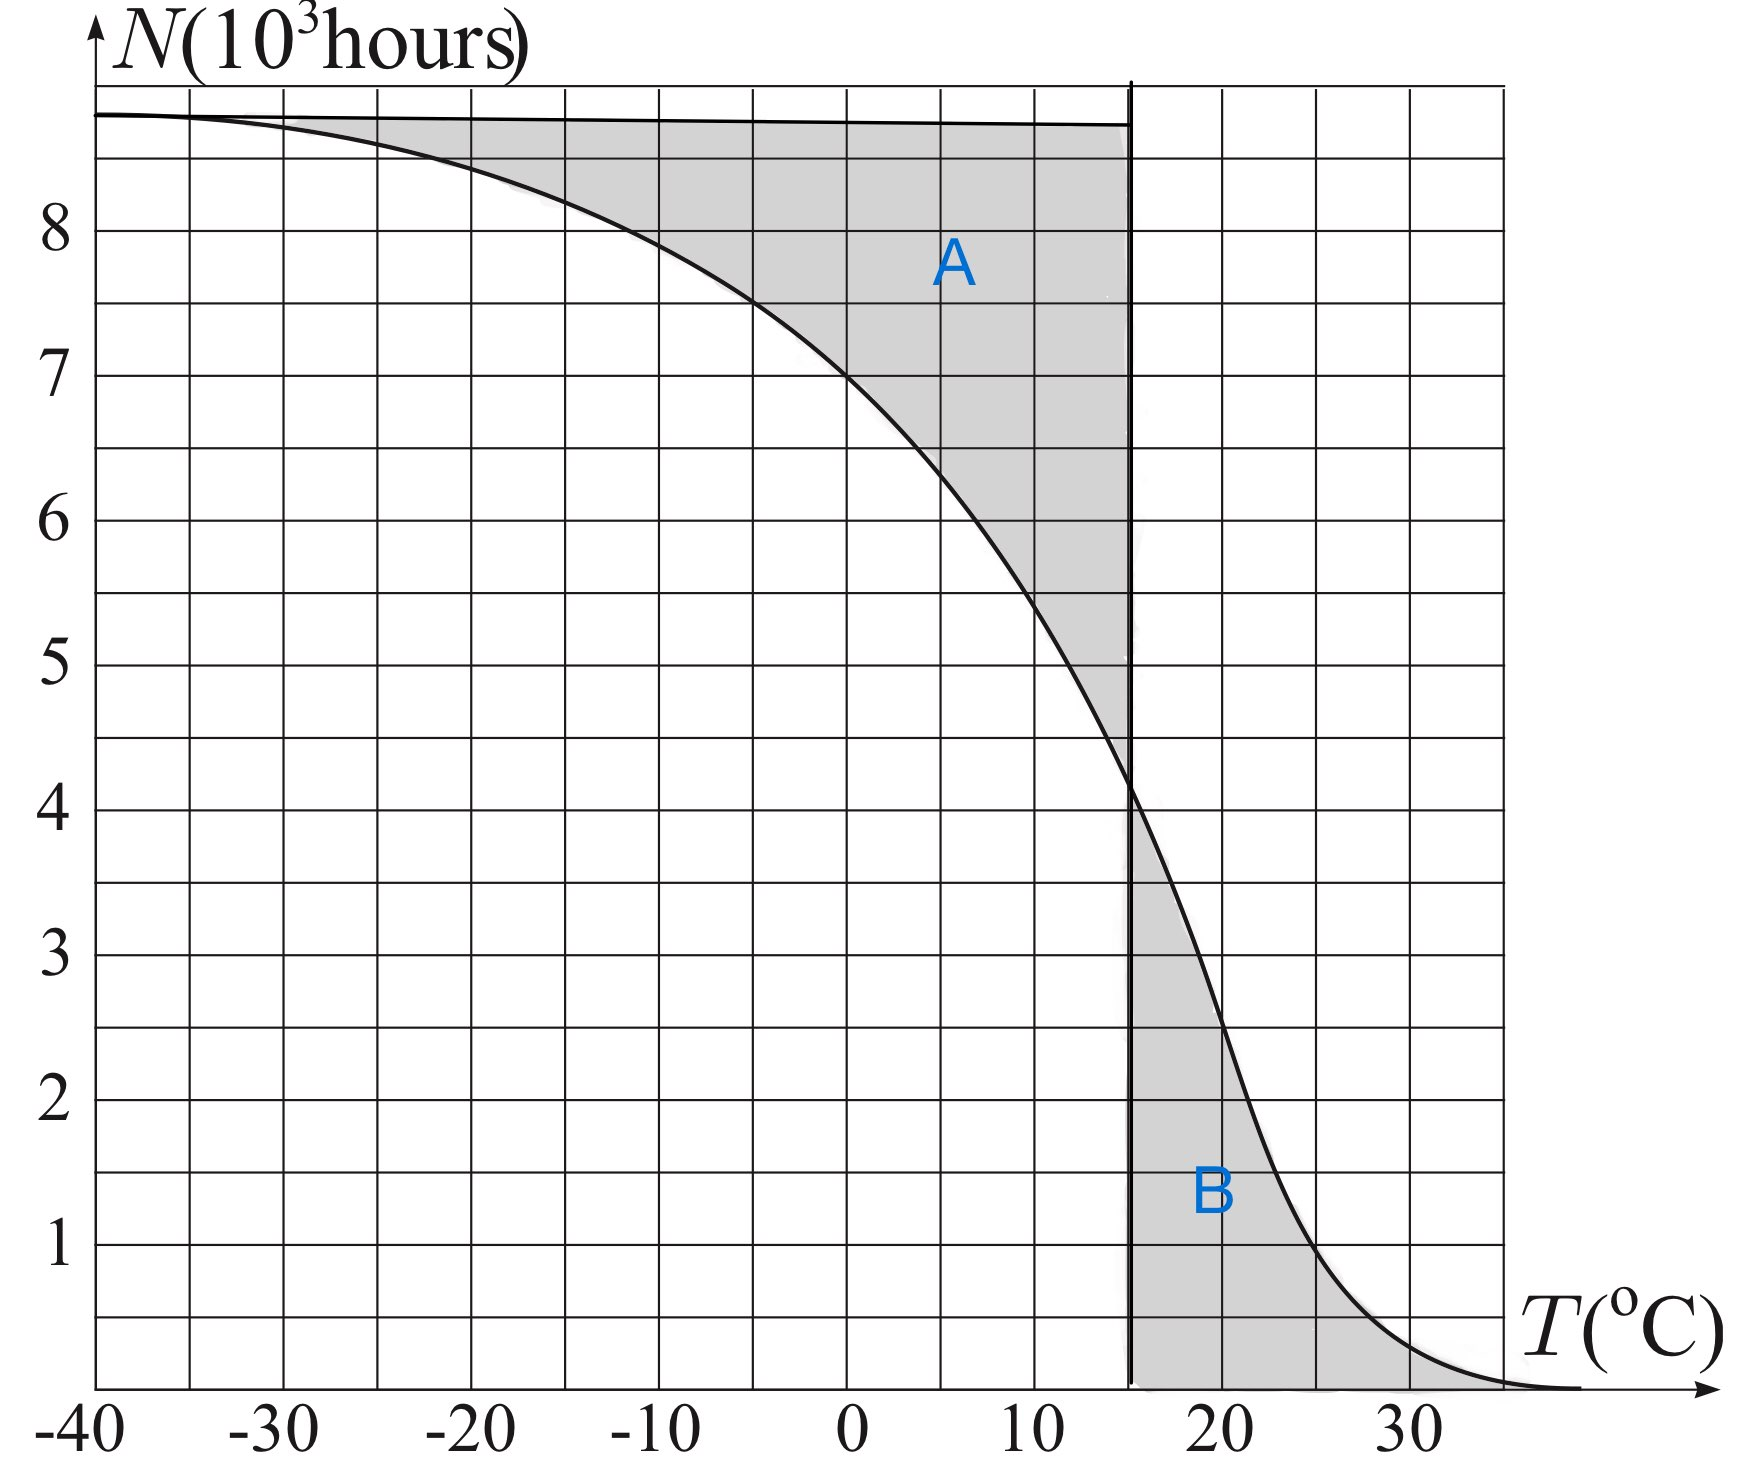
\includegraphics[width=10cm]{k46.jpg}
\end{center}
\end{solution}